\documentclass{article}
\usepackage[numbers]{natbib}
\usepackage[pagewise]{lineno}
%\linenumbers
%% AMS symbols
\usepackage{amssymb}

%% Geometry

\newcommand{\An}[1][n]{\ensuremath{\mathbb{A}^{#1}}} % Affine space
\newcommand{\Pn}[1][n]{\ensuremath{\mathbb{P}^{#1}}} % Projective space


%% Some common rings in maths.

\newcommand{\Complex}[0]{\ensuremath{\mathbb{C}}}
\newcommand{\Real}[0]{\ensuremath{\mathbb{R}}}
\newcommand{\Int}[0]{\ensuremath{\mathbb{Z}}}
\newcommand{\PadicInt}[1][p]{\ensuremath{\mathbb{Z}_{#1}}}
\newcommand{\PadicNum}[1][p]{\ensuremath{\mathbb{Q}_{#1}}}
\newcommand{\GF}[1][p]{\ensuremath{\mathbb{F}_{#1}}}
\newcommand{\Ideal}[1]{\ensuremath{\mathfrak{#1}}}


%% Quantum stuff

\newcommand{\ket}[1]{\ensuremath{\left\vert #1 \right\rangle}}
\newcommand{\bra}[1]{\ensuremath{\left\langle #1 \right\vert}}
\newcommand{\braket}[2]{\ensuremath{\left\langle #1 \vert #2 \right \rangle}}

%% Some common groups in maths

\newcommand{\GL}[2]{\ensuremath{\mathrm{GL_{#1}}\left(#2\right)}}
\newcommand{\SL}[2]{\ensuremath{\mathrm{SL_{#1}}\left(#2\right)}}
\newcommand{\PGL}[2]{\ensuremath{\mathrm{GL_{#1}}\left(#2\right)}}
\newcommand{\PSL}[2]{\ensuremath{\mathrm{GL_{#1}}\left(#2\right)}}
\newcommand{\Sym}[1]{\ensuremath{\mathrm{Sym}\left(#1\right)}}
%% Absolute values

\newcommand{\abs}[1]{\ensuremath{\left\vert#1\right\vert}}
\newcommand{\absp}[2][p]{\abs{#2}_{#1}}

%% Galois theory

\newcommand{\Gal}[1]{\ensuremath{\mathrm{Gal}\left(#1\right)}}

%% Algebraic complexity

\newcommand{\matrixtensor}[3]{\ensuremath{\left\langle #1,#2,#3 \right\rangle}}

%% Misc

\newcommand{\Perm}[1]{\ensuremath{\mathrm{perm}\left(#1\right)}}
\newcommand{\Det}[1]{\ensuremath{\mathrm{det}\left(#1\right)}}
\newcommand{\sgn}[1]{\ensuremath{\mathrm{sgn}\left(#1\right)}}
\newcommand{\transpose}[1]{\ensuremath{#1^{\mathrm{T}}}}
\newcommand{\Aut}[1]{\ensuremath{\mathrm{Aut}\left(#1\right)}}
\newcommand{\GI}[0]{\ensuremath{\mathrm{GI}}}
\newcommand{\AUT}[1][]{\ensuremath{\mathrm{AUT}_{#1}}}
\newcommand{\BCGI}[1]{\ensuremath{\mathrm{BCGI}_{#1}}}
\newcommand{\PWS}[1]{\ensuremath{\mathrm{PWS}_{#1}}}
 % Uncomment to get common commands
\usepackage{amsmath}
\usepackage{amssymb}
\usepackage{algorithm2e}
\usepackage{hyperref}

% To get theorem and other related environments

\usepackage{tikz}
\usetikzlibrary{positioning}
\usetikzlibrary{shapes}
\usetikzlibrary{backgrounds}
\usetikzlibrary{fit}
\usepackage{amsthm}
\newtheorem{theorem}{Theorem}[section]
\newtheorem{definition}[theorem]{Definition}
\newtheorem{lemma}[theorem]{Lemma}
\newtheorem{corollary}[theorem]{Corollary}
\newtheorem{proposition}[theorem]{Proposition}
\newtheorem{conjecture}[theorem]{Conjecture}
\newtheorem{observation}[theorem]{Observation}
\newtheorem{openproblem}[theorem]{Open problem}
\newtheorem{problem}[theorem]{Problem}
\newtheorem{remark}[theorem]{Remark}
\theoremstyle{remark}
\newtheorem{exercise}{Exercise}[section]
  % Uncomment to get theorem like stuff.


\title{Permutation groups and the graph isomorphism problem}
\author{Sumanta Ghosh and Piyush P Kurur\\
  Department of Computer Science and Engineering,\\
  Indian Institute of Technology Kanpur,\\
  Kanpur, Uttar Pradesh, India 208016\\
  {\tt \{smghosh,ppk\}@cse.iitk.ac.in}
}


\newcommand{\CP}[2]{\ensuremath{\mathrm{CP}\left(#1,#2\right)}}
\begin{document}
\maketitle
\begin{abstract}
  In this article, we discuss various algorithms for permutation group
  theoretic problems and study its close connection to the graph
  isomorphism problem. Motivated by this close connection, the last
  part of this article explores the \emph{group representability
    problem} and mention some open problems that arise in this
  context.

  \paragraph{Key words:} Graph isomorphism, permutation groups
\end{abstract}
\section{Introduction}

One of the core ideas in mathematics is the notion of an isomorphism,
i.e. structure preserving bijections between mathematical objects like
groups, rings and fields. A natural computational question is to
decide, given two such objects as input, whether they are isomorphic
or not. In the context of undirected finite graphs, this problem is
called the graph isomorphism problem and is the subject matter of this
article. Informally, we say that two graphs are isomorphic if they are
the same up to a renaming of their vertices, i.e. we have a bijection
between the vertex sets that preserve the adjacency relation of
edges. Many other isomorphism problems for explicitly presented finite
mathematical structures like groups, for example, reduce to the graph
isomorphism problem. Also, many problems that arise in practice, like
studying the structure of chemical compounds, are essentially graph
isomorphism in disguise. Hence, understanding this problem
computationally is important.

There are efficient programs and libraries (see
\href{http://pallini.di.uniroma1.it/}{NAUTY} for instance) that can
solve large instances of graph isomorphism that arise in
practice. However, there are no known polynomial-time algorithm for
the general case. In complexity theory, ever since the notion of
NP-completeness has been formalised, the graph isomorphism problem has
had an important status as it is believed to be a natural example of a
problem of intermediate complexity~\cite[Chapter 7]{garey-johnson},
i.e. neither in P nor NP-complete: It is know that the graph
isomorphism problem is in the complexity class
co-AM~\cite{boppana87does}, a randomised version of co-NP, and its NP
hardness will result in the collapse of the polynomial
hierarchy~\cite{boppana87does,schoning87graph}. Furthermore,
\citet{kobler92graph} showed that graph isomorphism is low for the
counting class PP by showing its membership in LWPP. This was further
improved by \citet{arvind2002graph} to SPP. As a result graph
isomorphism is in and low for various counting complexity classes like
classes like $\oplus \mathrm{P}$ etc. Thus, under reasonable
complexity theoretic assumptions, graph isomorphism is \emph{not}
NP-hard.  Ladner~\cite{ladner75ptimereduce} proved the existence of an
infinite hierarchy of problems of intermediate complexity assuming
that P is different from NP. The graph isomorphism problem, for
reasons stated above, is believed to be a natural example.

In this article, we study graph isomorphism and related
problems. There is now a vast literature on graph isomorphism and we
really cannot do justice to the topic in such a short article. For a
detailed study of graph isomorphism, mainly from a complexity
theoretic view point, we refer the reader to the excellent book by
\citet{gi-book}. This paper concentrates on one of the aspects of the
graph isomorphism problem, namely its intimate connection to
permutation group algorithms. Permutation groups arise in the study of
graph isomorphism problem because of its close relation to the graph
automorphism problem. For a graph $X$, the automorphisms,
i.e. isomorphisms from $X$ to itself, forms a group under function
composition. We can identify this group as a subgroup of the set of
all permutations of the vertex set $V(X)$. Automorphisms, thus are
symmetries of the graph. The computational problem of computing a
generating set of the automorphism group is equivalent to the graph
isomorphism problem~\cite{mathon79note}. Most algorithms for graph
isomorphism that make use of permutation group theory makes use of
this connection. Understanding the automorphism group of a graph is
also in tune with what is now a guiding principle in much of modern
mathematics: understanding objects by understanding their symmetries.

\section{Preliminaries}

We briefly review the group theory required for this article mainly to
fix notation and convention. For details please refer any standard
book on group theory, for example Marshall Hall~\cite{hall}. The
\emph{trivial group} that contains only the identity is denoted by
1. For a group $G$, we use the notation $H \leqslant G$ (or $G
\geqslant H$) to denote that $H$ is a subgroup of $G$. The \emph{right
  coset} of the subgroup $H$ of $G$ associated with an element $g\in
G$ is the set $Hg = \{ h g | h \in H\}$. The set of all right cosets
form a partition of $G$ and any subset $T$ of $G$ that has a unique
coset representative from each right coset is called a \emph{right
  transversal} of $H$ in $G$. Analogously, we define left cosets and
left transversals. In general, the right coset $Hg$ and the left coset
$gH$ are different. We say that $H$ is a \emph{normal subgroup} if $gH
= Hg$. We use the notation $H \unlhd G$ (or $G \unrhd H$) to denote
that $H$ is a normal subgroup of $G$.

A \emph{simple group} is a group that has no nontrivial normal
subgroups. A \emph{composition series} of a group $G$ is a tower of
subgroups $G = G_0 \unrhd G_1 \unrhd \ldots \unrhd G_t = 1$ such that
each of the factor groups $G_i/G_{i+1}$, called the \emph{composition
  factors}, are simple. The Jordan-H\"older theorem states that for
any group $G$, its composition series is essentially unique, i.e. any
two composition series are of equal length and the list of composition
factors are equal up to a reordering. \emph{Solvable groups} are those
whose composition factors are abelian.

The set of all permutation of $n$ elements forms a group called the
\emph{symmetric group} which we denote by $S_n$. In algorithmic
settings, it is often useful to make the domain of $n$ elements
explicit: For a finite set $\Omega$, the set $\Sym{\Omega}$ denote the
group of permutations on $\Omega$. By a \emph{permutation group} on
$\Omega$ we mean a subgroup of the symmetric group $\Sym{\Omega}$. As
is customary, we use Wielandt's notation~\cite{wielandt64finite}: Let
$\alpha$ be any element of $\Omega$ and let $g$ be a permutation in
$\Sym{\Omega}$, the image of $\alpha$ under $g$ is denoted by
$\alpha^g$. The advantage of this notation is that it follows the
familiar laws of exponentiation: $(\alpha^g)^h = \alpha^{gh}$. We can
extend this notation to (i) subsets of permutations: $\alpha^A =
\{\alpha^g | g \in A \}$, or to (ii) subsets of $\Omega$: $\Sigma^g =
\{ \alpha^g | \alpha \in \Sigma \}$. In particular, for a permutation
group on $\Omega$, the set $\alpha^G$ is called the \emph{$G$-orbit}
of $\alpha$. Given any two elements $\alpha$ and $\beta$ of $\Omega$
the $G$-orbits $\alpha^G$ and $\beta^G$ are either disjoint or are the
same. Thus, orbits of $G$ partition the underlying set $\Omega$. A
subset $\Sigma$ of $G$ is said to be \emph{$G$-stable} if $\Sigma^g =
\Sigma$. Clearly any $G$-orbit is $G$-stable. In general, a $G$-stable
set is a union of $G$-orbits.

Let $G$ be a permutation group acting on the set $\Omega$ and let
$\Sigma$ be a subset of $\Omega$. The \emph{point-wise stabiliser} of
$\Sigma$ is the subgroup of all $g$ in $G$ that is trivial on
$\Sigma$, i.e. $\alpha^g = \alpha$ for all $\alpha$ in $\Sigma$. The
\emph{setwise stabiliser} is the subgroup that fixes the set $\Sigma$
as a whole, i.e it is the subgroup of all $g$ in $G$ such that
$\Sigma^g = \Sigma$.

A permutation group $G$ is said to be \emph{transitive} if the entire
set $\Omega$ is a single orbit. Equivalently, $G$ is transitive if for
any two elements $\alpha$ and $\beta$ in $\Omega$ there is a
permutation $g$ in $G$ such that $\alpha^g = \beta$. For a transitive
permutation $G$ on $\Omega$, a subset $\Sigma$ is said to be a
\emph{$G$-block} if for any permutation $g$ in $G$, the set $\Sigma^g$
is either \emph{identical to} or \emph{disjoint from} the set
$\Sigma$. Any singleton set is a block and so is the entire set
$\Omega$. These blocks are called the \emph{trivial blocks} of $G$.
For a transitive permutation group $G$ on $\Omega$ and a permutation
$g$ in $G$, the set $\Sigma^g$ is a $G$-block whenever $\Sigma$ itself
is one.  Such a block $\Sigma^g$ is called a \emph{conjugate block} of
$\Sigma$. The family of conjugate blocks $\{ \Sigma^g | g \in G\}$
forms a partition of the set $\Omega$ which is called the \emph{block
  system} associated with the block $\Sigma$.  A permutation group
that has no nontrivial block is called a \emph{primitive permutation
  group}. An example of a primitive group is the group
$\Sym{\Omega}$. We have the following lemma about block systems which
is more or less direct from the definition.

\begin{lemma}\label{lem-block-g-action}
  Let $G$ be a transitive permutation group on $\Omega$ and let
  $\Sigma$ be a block. Let $N$ denote the subgroup of $G$ that setwise
  stabilises all the elements in the $\Sigma$-block system
  $\mathcal{B}(\Sigma) = \{\Sigma^g| g \in G \}$. Then $N$ is a normal
  subgroup of $G$ and $G/N$ acts as a permutation on $\Sigma$-block
  system $\mathcal{B}(\Sigma)$. In addition, if $\Sigma$ is a maximal
  $G$-block then this action of the group $G/N$ is primitive.
\end{lemma}

In algorithms that deal with permutation groups, we need a succinct
way to encode them which we now describe. Any permutation of $\Omega$
can be presented by an array of $\# \Omega$ elements and hence can be
encoded as a string of size $O(n \lg {n})$. A permutation group is
presented via a list of permutations that generate the group. It is a
well known fact that any group $G$ has a generating set of size less
than $\left\lceil\lg{\#G}\right\rceil$ and hence this presentation of
permutation group is reasonable. Thus, we assume that the input size,
for an algorithm that takes a generating set $S$ of a permutation
group $G$ on $\Omega$, is $\#S + \# \Omega$. Similarly, an algorithm
that is expected to produce a permutation group as output, should
output a generating set of size polynomial in $\# \Omega$. For
example, the strong generating set that we describe in the next
section, is of size at most $\# \Omega^2$.


By a graph we mean an undirected graph, i.e. a finite set of vertices
and an edge set which is a subset of unordered pairs of vertices. We
use $V(X)$ and $E(X)$ to denote the set of vertices and the set of
edges of a graph $X$ respectively. A bijection $f$ from $V(X)$ to
$V(Y)$ is an \emph{isomorphism} if for every two vertices $u$ and $v$
of $X$, the unordered pair $\{u,v\}$ is an edge of $X$ if and only if
$\{f(u), f(v)\}$ is an edge of $Y$. An \emph{automorphism} of a graph
$X$ is an isomorphism from the graph to itself. The set of
automorphism of a graph $X$, denoted by $\Aut{X}$, form a group under
composition. In fact, $\Aut{X}$ is a permutation group on $V(X)$.

In the article, we assume that a graphs of $n$ vertices is encoded as
an $n^2$-bit strings that represent its $n\times n$ adjacency
matrix. We now define the \emph{graph isomorphism problem}

\begin{problem}[Graph isomorphsim problem]
  The \emph{graph isomorphism problem} ($\GI$ for short) is defined as
  follows: Given two undirected graphs $X$ and $Y$ via their adjacency
  matrix, decide whether they are isomorphic.

  The counting version of the graph isomorphism problem, denoted by
  $\# \GI$, is the problem of computing the number of isomorphism
  between the two input graphs (0 when they are not isomorphic).
\end{problem}

Graph isomorphism problem is closely related to the \emph{automorphism
  problem} that we define next.

\begin{problem}[Automorphism problem]
  The \emph{automorphism problem} ($\AUT$ for short) is the problem of
  computing a strong generating set of the automorphism group
  $\Aut{X}$ of an input graph $X$.
\end{problem}



Mathon~\cite{mathon79note} proved that the problems $\GI$, $\# \GI$
and $\AUT$ are all polynomial-time Turing reducible to each
other. Therefore, in the setting of permutation group algorithms, it
is often the automorphism problem that is attacked for solving graph
isomorphism.

A graph $X$ is said to be \emph{rigid} if it has no nontrivial
automorphism, i.e. if $\Aut{X}$ is the trivial group. We now define
the graph rigidity problem.

\begin{problem}[Graph rigidity problem]
  Given an input graph $X$ via its adjacency matrix, check whether the
  graph is rigid.
\end{problem}

Clearly, an oracle for the automorphism problem, or by Mathon's
result~\cite{mathon79note}, the graph isomorphism problem, is
sufficient to decide the rigidity of a graph. However, the other
direction is open.

\begin{openproblem}
  Is the graph rigidity problem polynomial-time equivalent to the
  graph isomorphism problem.
\end{openproblem}


An important variant of graph isomorphism is the isomorphism of
coloured graphs.  For this article, a \emph{$c$-colouring} of a graph
$X$, where $c$ a positive integer, is a map from the vertex set $V(X)$
to the set of integers ${1,\ldots,c}$. Given a $c$-colouring $\psi$,
the $i$th \emph{colour class} is subset $\psi^{-1}(i)$ of $V(X)$. A
\emph{coloured graph} is a tuple $(X,\psi)$ of a graph $X$ and
colouring $\psi$. We often suppress the colouring $\psi$ when it is
understood from the context and just denote the coloured graph by
$X$. Given two $c$-coloured graphs $(X,\psi)$ and $(Y, \varphi)$, an
isomorphism $f$ between the underlying graphs $X$ and $Y$ is a
\emph{coloured graph isomorphism} if it respects the vertex colours,
i.e. for any vertex $v$ of $X$, $\psi(v)= \varphi(f(v))$. An
automorphism of a coloured graph is analogously defined. Clearly
coloured graph isomorphism generalises graph isomorphism as we can
assume an ordinary graph as 1-coloured graph. In the other direction,
coloured graph isomorphism polynomial-time Turing reduces to the graph
isomorphism problem. The key idea is the following \emph{gadget
  construction}. For a coloured graph $X$, we construct a new graph
$\tilde{X}$ by first adding, for each colour class $i$, a long path
$L_i$ (say of length $n + i + 1$). We then connect all the vertices of
the colour class $i$ to one of the end points of $L_i$. Given coloured
graphs $X$ and $Y$, any isomorphism between the modified graphs
$\tilde{X}$ and $\tilde{Y}$ forces the vertices in a given colour
class of $X$ to be mapped to the vertices of the same colour class in
$Y$ due to the graph gadgets $L_i$. Therefore, the coloured graphs $X$
and $Y$ are isomorphic if and only if the modified graphs $\tilde{X}$
and $\tilde{Y}$ are isomorphic. The rigidity problem and the
automorphism problem generalise naturally to coloured graphs as well.

The graph isomorphism problem and the automorphism problem can be
defined for directed graphs as well. It turns out that these variants
are polynomial-time Turing reducible to the undirected
case. Therefore, in this article, we mostly concentrate on undirected
graph isomorphism. Nonetheless, from the perspective of the
isomorphism problem, there is an important subclass of directed graphs
called \emph{tournaments} that we define below.

\begin{definition}
  A directed graph $X$ is a \emph{tournament} if for every two
  distinct vertices $u$ and $v$, exactly one of the directed edge
  $(u,v)$ or $(v,u)$ exists in $E(X)$.
\end{definition}

The automorphism group of a tournament cannot have a 2-cycle (why?),
and hence has to be of odd order. This forces it to be \emph{solvable}
by Feit-Thompson theorem~\cite{feit-thompson-theorem}. This property
has been exploited by \citet{babai83canonical} to give significantly
efficient algorithms for tournament isomorphism.


\section{Basic polynomial-time algorithms}

In this section, we mention some well known polynomial-time algorithms
for permutation group problems. The very first polynomial-time
algorithm is the algorithm to compute the orbits of a permutation
group. Let $S$ be a generating set of the permutation group $G$ then
define a relation $\alpha \rightarrow_S \beta$ if there exists a $g$
in $S$ such that $\alpha^g = \beta$. It is easy to see that the
symmetric, transitive closure of the relation $\rightarrow_s$ gives us
all the $G$-orbits. We can thus compute the orbits efficiently by
computing reachability.

\begin{lemma}
\label{lem:orbit_cal}
There is a polynomial-time algorithm, which given a generating set $S$
of a permutation group $G$ on $\Omega$ and an $\alpha \in \Omega$,
computes the orbit $\alpha^G$.
\end{lemma}

Many permutation group algorithms follows the general scheme of first
reducing the problem to the transitive case by finding all the orbits
of the group using the above lemma, and then restricting the group to
the orbit. This is followed by a divide can conquer that is done on
the blocks of the transitive action of the group. Thus, finding the
blocks of a transitive permutation group is a crucial step in various
algorithms. Let $G$ be a transitive permutation group over
$\Omega$. Fix any two elements $\alpha$ and $\beta$ in $\Omega$ and
consider the graph $X_{\alpha,\beta}$ whose vertices are $\Omega$ and
edges are $\{\alpha,\beta\}^G$. Let $\Sigma$ be the smallest $G$-block
containing both $\alpha$ and $\beta$ then Sim's observed~\cite{sims67}
that vertices in any connected component $C$ of the graph
$X_{\alpha,\beta}$ is a $G$-block in the block system $\{ \Sigma^g | g
\in G\}$ associated with $\Sigma$. By running this algorithm on all
pairs one can compute the set of minimal (as well as maximal) blocks
of $G$-blocks.

\begin{lemma}
  \label{lem:block_cal}
  There is a polynomial-time algorithm that takes as input the
  generating set of a transitive permutation group $G$ on $\Omega$ and
  decides whether $G$ is primitive or not. If the input group $G$ is
  not primitive, then it computes a minimal (or maximal) $G$-block
  system.
\end{lemma}

We already argued that a generating set of a group is a natural way to
present a permutation group. A \emph{strong generating set} is a
special generating set of a permutation group that makes many
computational tasks easy. Consider a permutation group $G$ on the set
$\Omega$. Fix an ordering $\{ \alpha_1,\ldots,\alpha_n\}$ on the set
$\Omega$ and let $G^{(i)}$ denote the subgroup of $G$ that fixes the
first $i$ elements of $\Omega$, i.e. the subgroup of all elements $g$
of $G$ such that $\alpha_j^g = \alpha_j$ for all $1 \leq j \leq
i$. Consider the \emph{tower} $G = G^{(0)} \geqslant \ldots \geqslant
G^{(n-1)} = 1$ of subgroups of $G$. Let $C_i$ be any set of
permutations that has exactly one element from each right coset of
$G^{(i)}$ in $G^{(i-1)}$, i.e. $C_i$ is a \emph{right transversal} of
$G^{(i)}$ in $G^{(i-1)}$. Given any permutation $g$ in $G$, there is
an unique element, say $h_1$, in $C_1$ which is in the same right
coset of $G^{(1)}$ as that of $g$. It is easy to see that $g' =
gh_1^{-1}$ is in $G^{(1)}$. Continuing this argument with $g'$ and the
group $G^{(1)}$, it is easy to see that any element $g$ can be
expressed as a product $h_1\ldots h_{n-1}$, $h_i\in C_i$. In fact, if
the transversals $C_i$'s are fixed, the above product representation
is unique. Thus, $\cup_i C_i$ forms a generating set of $G$ which we
call the \emph{strong generating} set of $G$.  Many computational
tasks become trivial once the strong generating set is calculated. For
example, the uniqueness of the product representation of $g$ shows
that the order of the group $\#G$ is the product of the sizes $\prod_i
\# C_i$.

We now describe the algorithm to compute the strong generating set of
a permutation group that was given in its complete form by
\citet{furst80polynomialtime} based on ideas from
\citet{sims78some}. It is based on the following lemma due to Schreier
and hence it (and similar algorithms) are some times called
\emph{Schreier-Sims algorithm}.

\begin{lemma}[Schreier's Lemma] \label{lem:schrier} Let $G$ be a group
  and $H$ be a subgroup of $G$. Let $T$ be any right transversal of
  $H$ in $G$ that contains $1$ as a coset representative. For each $g$
  in $G$, let $\overline{g}$ denote the unique coset representative of
  $Hg$ in $T$. Let $S$ be a generating set for $G$ then set
  \[ S' = \{ t s (\overline{ts})^{-1} | t,s \in S \} \] generates the
  group $H$
\end{lemma}

Let $S$ be the generating set of a permutation group $G$. The main
idea of the algorithm is that once we have a right transversal $C_1$
of $G^{(1)}$ in $G^{(0)} =G$, we can use Schreier's
Lemma~\ref{lem:schrier} to compute the Schreier generating set for
$G^{(1)}$. We then recursively compute the the strong generating set
for $G^{(1)}$. At each stage of the algorithm, we compute the right
transversal $C_{i+1}$ and recurse on the Schreier generating set of
$G^{(i+1)}$ obtained in that stage.

The right transversal $C_1$ is computed by starting with the set $T_0
= 1$ and inductively compute $T_{i+1}$ as follows: $T_{i+1}$ is the
union of $T_i$ and a subset of $T_iS$ such that $T_{i+1}$ does not
contain any redundant representative of same right coset of $G^{(1)}$,
i.e.  $T_{i+1}$ does not contain two distinct elements $g_1$ and $g_2$
such that $\alpha_1^{g_1}= \alpha_1^{g_2}$. If at some point $T_{i+1}
= T_i$, we stop the procedure. Since the set $C_1$ can at most have
$n$ elements this procedure has to terminate in polynomially many
steps. The actual algorithm~\cite{furst80polynomialtime} can be
significantly more efficient by computing all the transversals $C_i$'s
simultaneously through a sifting procedure. We summarise all the
polynomial-time solvable tasks that uses the Schreier-Sims procedure
in the following lemma.

\begin{lemma}[\citeauthor*{furst80polynomialtime}]
  \label{lem:order_member_subgrp_cal}
  There are polynomial-time algorithms for the computational tasks:

  \begin{enumerate}
  \item computing a strong generating set,
  \item computing the order of a permutation group,
  \item checking the membership of a permutation $g \in Sym(\Omega)$ in
    a given permutation group $G$.
  \end{enumerate}

\end{lemma}

The Schreier-Sims algorithm can be generalised to find the generating
set of a subgroup $H$ of a permutation group $G$, given indirectly by
a membership oracle, provided the index $\frac{\#G}{\# H}$ is
small. We state this in the next lemma.

\begin{lemma}\label{lem-general-schrier-sims}
  There is algorithm that takes as input a permutation group $G$ on
  $\Omega$ via a generating set $S$ and computes the generating set of
  a subgroup $H$ of $G$ given via a membership oracle, i.e. a
  procedure to test whether a given element $g$ of $G$ is actually an
  element of $H$. The algorithm takes time polynomial in $\# S$, $\#
  \Omega$ and the index $\frac{\# G}{\# H}$.
\end{lemma}

Consider a permutation group $G$ on $\Omega$ and let $\Delta$ be any
subset of $\Omega$. The \emph{point-wise stabiliser} of the set
$\Delta$, which we denote by $G(\Delta)$ is the subgroup of all
elements of $G$ that fix every element of $G$, i.e. $G(\Delta) = \{ g
| \delta^g = \delta,\ \forall \delta \in \Delta\}$. It is easy to see
that finding the point-wise stabiliser of any subset of $\Omega$ can
be done in polynomial-time by adapting the Schreier-Sims algorithm.

\section{Divide and conquer algorithms for permutation groups}

We now illustrate a general technique that is used in many permutation
group algorithms by giving an algorithm to find the setwise stabiliser
for special groups. Although superficially similar to point-wise
stabiliser, computing the setwise stabiliser is a different ball
game. It is at least as hard as graph isomorphism: For a graph $X$,
consider the group $G = \Sym{V(X)}$ acting on the set $\Omega = {V(X)
  \choose 2}$. The automorphism group of the graph $X$ is the set-wise
stabiliser of the subset $E(X)$ of $\Omega$. The setwise stabiliser
problem is a variant of a more general problem which we define below.

\begin{problem}[Colour preserving subgroup]
  Let $G$ be a permutation group on $\Omega$ which is partitioned into
  $k$-colour classes $\mathcal{C} = \{C_i \}_{i=1}^k$. Compute the
  subgroup of $G$ that stabilises each of the colour class $C_i$, i.e.
  compute the subgroup $\{ g \in G | C_i^g = C_i \}$
\end{problem}

The setwise stabiliser problem is the special case when the number of
colours is 2. While we cannot expect a polynomial-time algorithm for
this problem in general without solving the graph isomorphism problem,
for special groups, we can solve the above in polynomial-time. For
example, if we know that the input group $G$ is solvable then we have
a polynomial-time algorithm. In fact, the polynomial-time algorithm of
\citet{luks82bounded} for trivalent graphs uses such a subroutine as
the group that occurs there is a $2$-group and hence is solvable.

We now given a sketch of the algorithm, detail of which can be found
in the paper by \citet{luks82bounded}. To avoid notation clutter we
fix an input group $G$ and the colouring $\mathcal{C}$ of $\Omega$.
We say that a permutation $g$ preserves colours of all elements in the
subset $\Sigma$ if for all $\alpha \in \Sigma$, $\alpha$ and
$\alpha^g$ are in the same colour class. Let $H$ be a subgroup of $G$
and $\Sigma$ an $H$-stable subset of $\Omega$. We denote
$\CP{H}{\Sigma}$ to be the subset of $H$ that preserves the colours of
elements of $\Sigma$. Our task is to compute $\CP{G}{\Omega}$. For the
divide and conquer algorithm to work, we need to generalise the
problem to cosets of permutation groups: We need to compute
$\CP{Hg}{\Sigma}$ for the coset $Hg$ of the subgroup $H$ of $G$ where
the set $\Sigma$ is $H$-stable. Note that $\Sigma$ is not necessarily
stabilised by elements of $Hg$.

The set $\CP{Hg}{\Sigma}$ has the following crucial properties
which follows more or less directly from the definitions.

\begin{lemma}
  \begin{enumerate}
  \item The set $\CP{H}{\Sigma}$ is a subgroup of $H$.
  \item The set $\CP{Hg}{\Sigma}$ is either empty or is a coset of the
    group $\CP{H}{\Sigma}$.
  \item Suppose $\Sigma$ is the disjoint union $\Sigma_1 \uplus
    \Sigma_2$ both of which are $H$-stable then $\CP{Hg}{\Sigma} =
    \CP{\CP{Hg}{\Sigma_1}}{\Sigma_2}$.
  \end{enumerate}
\end{lemma}

It is crucial that $\CP{Hg}{\Sigma}$ is a coset (item 2 in the above
lemma) because we can then succinctly represent the set by giving a
generating set of $\CP{H}{\Sigma}$ and the coset representative.

We are now ready to give the outline of the divide and conquer
algorithm for computing $\CP{Hg}{\Sigma}$.

\begin{description}
\item[Reduction to transitive case] Let $\Sigma'\subset \Sigma$ be any
  $H$-orbit. We first compute the group $\CP{Hg}{\Sigma'}$ which is
  the transitive case of the above problem.  Let $\Sigma = \Sigma'
  \uplus \Sigma''$. We use the fact that $\CP{Hg}{\Sigma} =
  \CP{\CP{Hg}{\Sigma'}}{\Sigma''}$.
\item[Transitive case] For this case $H$ acts transitively on
  $\Sigma$. Let $\Delta$ be a \emph{maximal} $H$-block of $H$ and let
  $\mathcal{B}(\Delta) = \{ \Delta_1, \ldots, \Delta_k\}$ be the
  associated block system. Let $N$ be the normal subgroup of $H$ that
  fixes all the blocks $\mathcal{B}(\Delta)$ setwise. Then we have $H
  = \uplus_x N x$ as a disjoint union of cosets of $N$. We can then
  compute the set $\CP{Hg}{\Sigma}$ by taking the union of all the
  cosets $\CP{Nxg}{\Sigma}$ which are not empty.
\end{description}

If the number of cosets $Nx$ are polynomially bounded then we can
compute a generating set for $N$ using
Lemma~\ref{lem-general-schrier-sims}. It then amounts to recursively
computing the polynomially many cosets $\CP{Nxg}{\Sigma}$ and
combining the non-empty ones. The number of cosets $Nx$ that is
considered in the transitive case is the same as the order of the
quotient group $H/N$. Since the block $\Delta$ that we choose is the
maximal block, the quotient group $H/N$, as a permutation group on the
set $\mathcal{B}(\Delta)$, is a primitive group
(See~\ref{lem-block-g-action}). Thus, we need a bound on the size of a
primitive permutation group. While the order of a primitive
permutation group on $n$ elements can be exponential in $n$, consider
the case of the primitive group $S_n$ for example, for solvable
primitive permutation groups, a result by P\'alfy~\cite[Theorem
1]{palfy82primitive} gives us the polynomial bound we are looking for.

\begin{theorem}[\citeauthor{palfy82primitive}]\label{thm-palfy}
  There are absolute constants $C$ and $c$ such that any solvable
  primitive permutation group on $\Omega$ is of size less than $C
  \cdot \# \Omega^c$.
\end{theorem}

The above bound has a generalisation to groups with bounded
non-abelian composition factors: Let $\Gamma_d$ denote the class of
groups such that each composition factor is either abelian or is
isomorphic to a subgroup of $S_d$. \citet{babai82primitive}
generalised the P\'alfy's bound to the class $\Gamma_d$.

\begin{theorem}[\citeauthor*{babai82primitive}]\label{thm-palfy-gen}
  There are absolute constants $C$ and $c$ such that for any positive
  integer $d$, any primitive permutation group on $\Omega$ in the
  class $\Gamma_d$ is of size less than $C\# \Omega^{c d}$.
\end{theorem}

As a result, the colour preserving subgroup problem is solvable in
polynomial-time for groups that are in the class $\Gamma_d$.

\begin{lemma}\label{lem-colour-preserving-algo}
  Colour preserving subgroup problem is solvable in polynomial-time
  for the class of solvable groups and the class of groups in the
  family $\Gamma_d$ for constant $d$.
\end{lemma}


We now discuss a natural context where the colour stabiliser problem
for groups in the class $\Gamma_d$ occurs. Consider the graphs of
valence $d$, i.e. all vertices are of degree less than or equal to
$d$. Luks~\cite{luks82bounded} gives a polynomial-time algorithm for
this class of graphs by reducing it to the colour preserving subgroup
problem where the input group $G$ is in the class $\Gamma_{d-1}$. We
quickly give a sketch.

Fix the two input graphs graphs $X_1$ and $X_2$. We assume that the
graphs are connected, otherwise we run the algorithm for each pair of
connected components. Furthermore, we restrict our attention to
checking whether $X_1$ and $X_2$ are isomorphic via an isomorphism
that maps a particular edge $e_1$ of $X_1$ to an edge $e_2$ of $X_2$:
We just need to repeat the procedure for all such pairs of edges to
know whether $X_1$ and $X_2$ are isomorphic.
\begin{figure}
  \hfil
  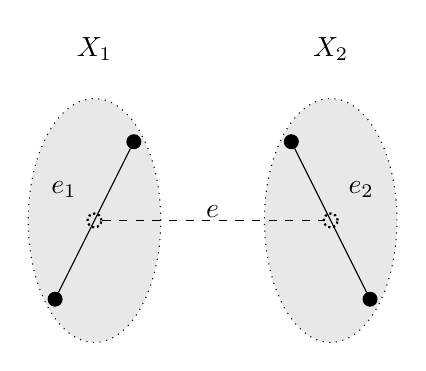
\begin{tikzpicture}
    [ inner sep=0pt,
    every node/.style={circle, minimum size=5pt},
    O/.style={fill=black,draw},
    o/.style={densely dotted,draw, thick},
    distance=0.5cm,
    graph/.style={shape=ellipse, fill=black!10!white!90}
    ]

    \pgfdeclarelayer{background};
    \pgfsetlayers{background,main};


    \node[O] (u0) at (0,0) {};
    \node[o] (u)  at (0.5,1) {};
    \node[O] (u1) at (1,2) {};

    \node[O] (v1) at (3,2) {};
    \node[o] (v)  at (3.5,1) {};
    \node[O] (v0) at (4,0) {};

    \draw [-] (u0) -- node [label, above left=10pt]{$e_1$} (u1);
    \draw [-] (v0) -- node [label, above right=10pt]{$e_2$} (v1);
    \draw [dashed] (u) -- node [label, above]{$e$} (v);



    \begin{pgfonlayer}{background}
      \node[graph, dotted, draw, fit=(u0) (u) (u1)](X1){};
      \node[graph, dotted, draw, fit=(v0) (v) (v1)](X2){};
    \end{pgfonlayer}

    \node [above=10pt of X1.north] {$X_1$};
    \node [above=10pt of X2.north] {$X_2$};
  \end{tikzpicture}\hfil
  \label{fig-bounded-valence}
  \caption{Luks gadget for bounded valence graphs}
\end{figure}

Consider the new graph which we denote by $Z$ which is essentially the
disjoint union of the graph $X_1$ and $X_2$ with an additional edge
$e$ that connects the mid points of $e_1$ and $e_2$ (see
figure~\ref{fig-bounded-valence}). If $d>2$ is the maximum degree of
any vertex in the input graph then $Z$ also has degree bounded by
$d$. Luks algorithm for bounded valence computes the group subgroup
$\Aut{Z}_e$ of $\Aut{Z}$ that maps the auxiliary edge $e$ to
itself. It is clear that the input graphs $X_1$ and $X_2$ are
isomorphic if and only if there is at least one element in $\Aut{Z}_e$
(and therefore in any generator set) that flips the edge $e$. The
algorithm then proceeds to compute the group $\Aut{Z}_e$. First the
graph $Z$ is layered as follows: Let the $i$th layer of $Z$, denoted
by $Z_i$, be the sub graph which contains all the edges (as well as
the end points) at a distance $i$ from the auxiliary edge $e$. In
particular, the graph $Z_0$ consists of just the edge $e$ and its end
points. All automorphisms of $Z$ that stabilises the edge $e$ has to
preserve this layered structure. The group $\Aut{Z}_e$ is then
computed by inductively computing the groups $G_i=\Aut{Z_i}_e$.

Inductively, Luks proves that $G_i$'s are in the class $\Gamma_{d-1}$
as follows: Let $H_{i+1}$ denote the subgroup of $G_i$ that is
obtained by restricting elements of $G_{i+1}$ on $Z_i$ and let
$K_{i+1}$ be the associated kernel, i.e. the subgroup of $G_{i+1}$
that is trivial when restricted to $Z_i$. Any vertex $u$ in layer $i$,
i.e. in the graph $Z_i\setminus Z_{i-1}$, is connected to at most
$d-1$ vertices in the layer $i+1$ and these vertices have to be mapped
within themselves by elements of $K_{i+1}$. Therefore, $K_{i+1}$ is a
subgroup of a product of $m$ many copies of the symmetric groups
$S_{d-1}$ for some positive integer $m$. The quotient group
$G_{i+1}/K_{i+1}$ is the group $H_{i+1}$, which itself is a subgroup
$G_i$, a group in the class $\Gamma_{d-1}$. This is possible only if
$G_{i+1}$ is in $\Gamma_{d-1}$: Consider any composition series of
$G_{i+1}$ which passes through the normal subgroup $K_{i+1}$. The
composition factors are either composition factors of $H_i$ or that
$K_{i+1}$.

Having computed $G_i$ the algorithm computes $G_{i+1}$ by computing
(1) a generating set for the kernel $K_{i+1}$ and (2) a set of
elements of $G_{i+1}$ whose restriction to $G_i$ generates $H_i$. It
is this inductive step that requires the solution of colour preserving
subgroup problem and luckily the input group ($G_i$ in our case) turns
out to be in the class $\Gamma_d$ and hence solvable by the algorithm
in Lemma~\ref{lem-colour-preserving-algo}. Thus we have the following
theorem.

\begin{theorem}[Luks]
  Consider the family $\mathcal{G}_d$ of graphs whose vertices are of
  degree bounded by $d$. There is a $n^{O(d)}$ algorithm to decide
  isomorphism of graphs in $\mathcal{G}_d$.
\end{theorem}

The current fastest algorithm for graph
isomorphism~\cite{zemlyachenko85gi} is based on a valence reduction
step together with the application of the above theorem of Luks for
bounded valence graphs. Therefore, any improvement on the bounded
valence case will improve the state of the art for the general graph
isomorphism problem.

\section{Lexicographically least permutations}

We now mention some results that make use of the ordering of
permutations induced by the ordering on the domain $\Omega$. Firstly
note that a total ordering on the set $\Omega$ gives a total ordering
on $\Sym{\Omega}$: for distinct permutations $g$ and $h$, $g < h$ if
at the first (in the ordering on $\Omega$) element $\alpha$ in
$\Omega$ where they differ, we have $\alpha^g < \alpha^h$. We call
this ordering the \emph{lexicographic ordering} on the
permutations. Under this ordering the lexicographically least
permutation is the identity permutation. The first problem that we
study is the problem of computing the lexicographically least element
in a coset.

\begin{problem}[lexicographically least in a coset]
  Given a permutation group $G$ on $\Omega$ as a set of generators and
  an arbitrary permutation $x$ on $\Omega$, compute the
  lexicographically least element in the coset $Gx$.
\end{problem}

Clearly if $x$ is in $G$ then the coset is the group $G$ itself and
the lexicographically least element of the coset is the identity
element. We now sketch a polynomial-time algorithm for this problem.

Let $\alpha$ be the least element of $\Omega$. The set of images of
$\alpha$ under permutations in the coset $Gx$ is given by the set
$\alpha^{Gx} = (\alpha^G)^x$ which can be computed easily once the
orbit $\alpha^G$ of $\alpha$ is computed. Clearly, the
lexicographically least element of $Gx$ should map $\alpha$ to the
least element $\beta$ of $\alpha^{Gx}$. We can also compute, using the
transitive closure algorithm for orbits, an element $x_1$ in the coset
$Gx$ such that $\alpha^{x_1} = \beta$. Therefore the lexicographically
least element of $Gx$ is also the lexicographically least element in
the coset $G_\alpha x_1$ as this coset is precisely the set of
elements of $Gx$ that maps $\alpha$ to $\beta$. A similar algorithm
can be give for left cosets $xG$ as well. We thus have the following
lemma:

\begin{lemma}
  Computing the lexicographically least element in a coset can be done
  in polynomial-time.
\end{lemma}

The above lemma is a key step in proving that the graph isomorphism
problem is in the complexity class SPP.

\begin{definition}[SPP]
  For a non-deterministic polynomial-time Turing machine let
  $\mathrm{gap}(M,x)$ denote the \emph{difference} in the number of
  accepting paths and rejecting paths of $M$ on the input $x$.  A
  language $L$ is in the complexity class \textrm{SPP} if there is a
  polynomial time non-deterministic Turing machine $M$ such that for
  all strings $x$ in the language $L$, the $\mathrm{gap}(M,x)$ is 1
  and for all strings not in the language $L$, $\mathrm{gap}(M,x)$ is
  0.
\end{definition}

Languages in SPP are believed to be of low complexity and are unlikely
to be NP-hard. In particular, any \emph{gap definable
  complexity}~\cite{fenner91gapdefinable} class not only contain SPP
but also derive no extra computational power with a language in SPP as
oracle, i.e. SPP is \emph{low} for all these complexity classes. Gap
definable complexity classes~\cite{fenner91gapdefinable} are counting
classes defined using GapP functions, i.e. functions that are
differences of accepting and rejecting paths of an NP machine, and
contain many common counting complexity class like PP and
$\oplus\mathrm{P}$ etc.

The main idea involved in the proof is to design a polynomial-time
algorithm $A$ that makes queries to an NP language $L$ with some
restriction on the queries that $A$ makes to $L$. We design a
non-deterministic polynomial time machine $M$ for $L$ such that for
all queries the algorithm $A$ makes, the machine $M$ has at most one
accepting path. Such an oracle machine can be converted to an SPP
algorithm, i.e. an NP machine whose gap function is the characteristic
function of GI, using standard techniques~\cite{kobler92graph}.

The base algorithm $A$ is an inductive algorithm that builds the
strong generating set of the automorphism group by computing the group
$G_i$ of all automorphisms that fix the first $i$ vertices of the
graph. To compute $G_{i-1}$ from $G_i$, the algorithm has to query the
NP-language $L$ which essentially checks, given a $j> i$, whether
there is an automorphism that maps $i$ to $j$.  The base
polynomial-time machine can then find one such by doing a prefix
search. However, we need to design an NP machine $M$ for $L$ such that
for all queries asked by $A$, there is at most one accepting
path. This we achieve as follows: The algorithm $A$ also provides to
$L$ the generator set of $G_i$, i.e. queries to $L$ are (encoding of)
pairs $\langle S,j\rangle$ where $S$ is a generating set of $G_i$ at
the $i$-th stage. We know that if there is an automorphism, say $g$ in
$G_{i-1}$, that maps $i$ to $j$ then the set of all such automorphisms
form the coset $G_i g$. The machine $M$ essentially guess the
automorphism $g$ that maps $i$ to $j$ if it exists and accepts only if
$g$ is the lexicographically least permutation in $G_ig$. Since there
is only one such guess $g$, we know that for all queries that the
algorithm $A$ makes to $L$ the machine $M$ has at most one accepting
path. The SPP result then follows as mentioned above.

\begin{theorem}[Arvind and Kurur]
  The graph isomorphism problem is in SPP.
\end{theorem}

While computing the lexicographically least element in a coset has an
efficient algorithm, consider the following generalisation to a double
coset.

\begin{problem}[Lex-least in a double coset]
  Given the generating sets of permutation groups $G$ and $H$ on a
  totally ordered set $\Omega$ and an arbitrary permutation $x$ on
  $\Omega$, compute the lexicographically least element in $GxH$.
\end{problem}

The problem of computing the lex-least element in a double coset is
intimately connected to the problem of graph canonisation which we
define below.

\begin{definition}[Canonical forms for graphs]
  Consider the class $\mathcal{G}(\Omega)$ of all graphs on the vertex
  set $\Omega$. A function $\mathbf{CF}$ on $\mathcal{G}(\Omega)$ is a
  \emph{canonical form} if it satisfies the following properties:
  \begin{enumerate}
  \item For every graph $X$ in $\mathcal{G}(\Omega)$, $\mathbf{CF}(X)$
    is isomorphic to $X$.
  \item If $X$ and $Y$ are two isomorphic graphs then $\mathbf{CF}(X)$
    is the same as $\mathbf{CF}(Y)$.
  \end{enumerate}
\end{definition}

In other words, a canonical form $\mathbf{CF}$ picks a unique
representative from each isomorphism class of graphs on
$\Omega$. Clearly graph isomorphism is solvable given a canonisation
procedure. Therefore, one way of attacking the graph isomorphism
problem is to give fast canonisation procedure. For many classes of
graphs, Babai and Luks~\cite{babai83canonical} gave an efficient
canonisation procedure which is also currently the best general
purpose algorithms. In particular, they were able to give an
$O\left(n^{c \log{n}}\right)$ for tournaments. This canonisation
procedure makes use of the fact that tournaments have a solvable
automorphism group. They also show how Luks' polynomial-time algorithm
for bounded valance~\cite{luks82bounded} can be modified and extended
to a canonisation algorithm with essentially the same running time.

As opposed to computing the lexicographically least element in a
coset, computing it in a double coset is known to be
NP-hard~\cite[Theorem 5.1]{luks93permutation} even when one of the
group is solvable. However, in many contexts, particularly in relation
with graph isomorphism and canonisation, we have some freedom to
choose the underlying ordering of the set $\Omega$. Can we reorder the
set $\Omega$ so as to make it possible to apply the divide and conquer
technique similar to that of the colour preserving subgroup problem
that we saw in the previous section?  Indeed this is the case provided
the reordering is ``compatible'' with the divide and conquer structure
of the group $G$. Firstly, we need to generalise the lexicographically
least element as follows: Consider an ordering $<$ on $\Omega$. Let
$\Delta$ be a $G$-stable set. We consider the restriction of the order
$<$ on the set $\Delta$. This gives a partial order on elements of
permutations, we say that $g < h$ if for the least $\delta$ in
$\Delta$ on which $g$ and $h$ differ, we have $\delta^g <
\delta^h$. Under this restricted ordering there will be multiple
lexicographically minimal elements. We now describe how to build a new
ordering $\prec$ on $\Omega$ under which it is feasible to compute the
lexicographically least element of the double coset $GxH$.


\begin{description}
\item[Ordering the orbit] Fix an ordering between the $G$-orbits by
  picking say the least element in each of them. If $\Omega_1$ and
  $\Omega_2$ are two orbits such that $\Omega_1 < \Omega_2$ in the
  above chosen order, then we set every element of $\Omega_1$ to be
  less than that of $\Omega_2$ under the new ordering $\prec$. The
  motivation of this reordering is the following: Let $\Omega =
  \Omega_1 \uplus \Omega_2$ then computing the lexicographically least
  element with respect to the new ordering $\prec$ can be done by
  first computing the lexicographically minimal elements with respect
  to the restriction of $\prec$ on $\Omega_1$ and then from them
  picking the lexicographically least element with respect to the
  restriction of $\prec$ on $\Omega_2$.

\item[Ordering within orbits] When $G$ is transitive, we do the
  reordering with respect to the blocks. We pick a maximal $G$-block
  $\Delta$ in a canonical way. The $\Delta$ block system partition the
  set $\Omega$ so reorder it pretty much the same way as in the
  previous case using the $\Delta$ block system instead. If $N$
  denotes the normal subgroup of $G$ that fixes all the blocks in the
  $\Delta$ block system, we can recursively find the lex-least
  elements in double cosets $NgxH$ and find the minimal ones out of
  it. If $G$ is in the class $\Gamma_d$, the number of sub-problems
  are polynomially bounded by Theorem~\ref{thm-palfy-gen}.
\end{description}

The above reordering can be formalised in terms of the \emph{structure
  forest} of the group $G$. The structure forest is the collection of
\emph{structure trees} one for each $G$-orbit. For an orbit $\Sigma$,
the structure tree is a tree where the leaves are elements of
$\Sigma$.  Each internal node $v$ is associated with a $G$-block
$\Delta_v$ with the following properties.

\begin{enumerate}
\item For any child $u$ of $v$, the $G$-block $\Delta_u$ is a maximal
  block contained in $\Delta_v$.
\item If $\{u_1,\ldots, u_k\}$ are the set of children of $v$ then the
  blocks $\Delta_{u_i}$'s are all conjugates of each other and
  partition the parent block $\Delta_v$.
\end{enumerate}

This structure forest captures the divide and conquer on $G$. The
elements of $\Omega$ can be reordered once we compute the structure
forest of $G$: The structure trees are ordered in the order of the
least element in them. For each internal node $v$ and children $u_1$
and $u_2$, $u_1 \prec u_2$ if the least element of the associated
block in $u_1$ is smaller than that of $u_2$ according to the original
ordering $<$. This will finally give an ordering $\prec$ on the entire
set $\Omega$. Thus, we have the following theorem (See the survey
article by Luks~\cite{luks93permutation} for details).

\begin{theorem}
  Given a totally ordered set $\Omega$, permutation groups $G$ and $H$
  on $\Omega$ and a permutation $x$ on $\Omega$. Suppose $G$ is in the
  class $\Gamma_d$ then in time polynomial in $n$ we can compute a new
  ordering $\leq_G$ such that computing the lex-least element of the
  double coset $GxH$ can be done in $n^{O(d)}$.
\end{theorem}

Notice that we do not have any restriction whatsoever on the group
$H$.

\section{Structure of primitive groups}

In the last two sections, we saw how bounds on the order of primitive
permutation group can be crucial in the runtime analysis of various
divide and conquer algorithms for permutation groups. We now mention
how knowing the actual structure of primitive groups are
computationally useful. This section is mainly motivated by the study
of \emph{bounded colour class graph isomorphism problem}.

\begin{problem}[Bounded colour class graph isomorphism]
  Fix a constant $b$. Given two coloured graph $X$ and $Y$ such that
  the number of vertices in any given colour class is bounded by $b$
  decide whether the graphs are isomorphic.
\end{problem}

We abbreviate this problem as $\BCGI{b}$. This restricted graph
isomorphism problem does have polynomial-time algorithm but what about
fast parallel algorithms?  \citet{luks86parallel} answered this
question affirmatively by giving a reduction to a restricted
point-wise stabiliser problem and solving it in NC. Further careful
analysis by \citet{arvind2005bounded} showed that the problem lies in
the $\mathrm{Mod}_k\mathrm{L}$ hierarchy. Together with the hardness
for this class~\cite{toran2004hardness}, we have a fairly tight
classification of this variant of graph isomorphism.

We now explain the overall structure of the algorithm for
$\BCGI{b}$. Both \citet{luks86parallel} and \citet{arvind2005bounded}
reduce the bounded colour graph isomorphism problem to a restricted
version of point-wise stabiliser problem which we now define.

\begin{problem}[bounded orbit point-wise stabiliser problem]
  Given as input a set $\Omega$, a subset $\Delta$ of $\Omega$ and a
  permutation group $G$ on $\Omega$ such that the $G$-orbits are all
  of cardinality bounded by a constant $c$.  Compute generating set of
  the point-wise stabiliser subgroup $G(\Delta)$.
\end{problem}

We abbreviate this problem as $\PWS{c}$. As mentioned before, the
above problem is solvable in polynomial-time.  However, in this
context, we are interested in providing a parallel algorithm. What
needs to be exploited is that the $G$-orbits are bounded and thus $G$
is actually a subgroup of a product of small symmetric groups, the
symmetric groups on each of the $G$-orbits.

To see the connection of the $\PWS{c}$ and $\BCGI{b}$ isomorphism we
consider the equivalent automorphism problem which we denote by
$\AUT[b]$.

\begin{lemma}[\citeauthor{luks86parallel}]
  The $\AUT[b]$ problem logspace reduces to $\PWS{2^{b^2}}$ problem.
\end{lemma}

Here is the sketch of this reduction. Let $X$ be the coloured graph
and let $C_1,\ldots, C_m$ denote the the colour classes into which the
vertex set $V(X)$ is partitioned. The automorphism group is a subgroup
of the product group $G = \prod_{i}\Sym{C_i}$. We expressed the
automorphism group $\Aut{X}$ as a point-wise stabiliser of $G$ on its
action on a different set $\Omega$ that we construct as follows:
Define the set $C_{i,j}$ to be the set of unordered pairs $\{u,v\}$
where $u\in C_i$ and $v \in C_j$ and let $E_{i,j}$ be the subset of
edges of $X$ between the colour classes $C_i$ and $C_j$. Define the
set $\Omega_{i,j}$ to be the power set of $C_{i,j}$ then the edge sets
$E_{i,j}$ are actually \emph{points} or element of
$\Omega_{i,j}$. Consider the natural action of $G$ on the union
$\Omega = \cup_{i,j} \Omega_{i,j}$ and let $\Delta$ be the subset of
all the \emph{points} $E_{i,j}$ of $\Omega$. It is easy to see that
the point-wise stabiliser of $G$ with respect to the subset $\Delta$ is
actually the automorphism group $\Aut{X}$. Notice that each of the set
$\Omega_{i,j}$ are $G$-stable and hence the orbits of $G$ are at most
of size $2^{b \choose 2}$.

Both \citet{luks86parallel} and \citet{arvind2005bounded} then solve
the $\PWS{c}$ problem.  While the actual algorithms of
\citet{luks86parallel} and \citet{arvind2005bounded} are fairly
technical, we attempt to explain the essence of the algorithm and the
permutation group theory involved in those results.

The group $G$ in question can be seen as a product of groups $G =
\prod_i G_i$ where $G_i$ is the action of $G$ on the $i$th orbit. For
each of the groups $G_i$, compute a special \emph{normal series} $G_i
= N_{i,0} \rhd \ldots \rhd N_{i,t}$ and let $N_k$ denote the produce
$\prod_i N_{i,k}$. The algorithm does a divide and conquer to compute
$N_k(\Delta)$ going one level at a time. The base case of this divide
and conquer is when the group $N_{i,s}$ hits a socle. The \emph{socle}
of a group $G$ is the group generated by the set of all minimal normal
subgroups of $G$.  The main group theoretic result that is used is the
O'Nan-Scott theorem (See the book by~\citet{dixon91permutationbook}
for a proof of this result) on the structure of the socle of a
primitive permutation group and its point-wise stabiliser.

% \begin{theorem}[O'Nan-Scott]
%   Let $G$ be primitive permutation group on $\Omega$ then its socle
%   $K$ is a product of isomorphic copies of a single simple group $T$.
%   Furthermore, the group $K$ can be any of the following three cases.

%   \begin{enumerate}
%   \item $K$ is abelian in which case the point-wise stabiliser
%     $K_\alpha$ for any element $\alpha$ in $\Omega$ is trivial.
%   \item $K$ is non-abelian and the unique minimal normal subgroup of
%     $G$.  For each $\alpha$ in $\Omega$, the point-wise stabiliser
%     $K_\alpha$ is a proper subgroup of $K$
%   \item $K$ is non-abelian and is the product $K_1 \times K_2$ of two
%     isomorphic subgroups $K_1$ and $K_2$ both of which are minimal
%     normal subgroups of $G$. The point-wise stabiliser $K_\alpha$ is a
%     diagonal of the product $K_1 \times K_2$.
%   \end{enumerate}

% \end{theorem}

For the details of the algorithm, we refer the reader to the
conference paper of \citet{arvind2005bounded}. A detailed version is
available in the Ph.D thesis of \citet[Chapter 5]{K2006}

\section{Representation of groups on graphs}

In this section, we look at the group representability problem. This
problem was defined and studied by \citet{kurur09} to explore the
connection between graph isomorphism and permutation group algorithms
from a representation theoretic point of view. Representation theory
is the study of homomorphisms from a group to the group
$\mathrm{GL}(V)$, the automorphisms of a vector space $V$. In the
context of graph isomorphism, we would like to understand
homomorphisms between groups and automorphisms of graphs.

\begin{definition}
  A \emph{representation} of a group $G$ \emph{on a} graph $X$ is a
  homomorphism from the group $G$ to the automorphism group $\Aut{X}$
  of the graph $X$. 
\end{definition}

There is always a trivial representation that sends all the elements
of the group to the identity automorphism. What we are interested in
is a non-trivial homomorphisms. The main problem of interest in this
section is the following~\cite{kurur09}.

\begin{problem}[Group representability problem]
  Given a group $G$ and a graph $X$, decide whether $G$ has a
  non-trivial representation on $X$.
\end{problem}

The hardness of the problem depends on how the group $G$ is
presented. We assume, unless otherwise mentioned, that $G$ is provided
to the algorithm via a multiplication table. Therefore, one can assume
that the input size is $\# G + \# V(X)$. In studying its connection to
graph isomorphism, we can restrict the problem in two ways: (1)
restrict the groups to come from a natural class like for example
solvable or abelian or (2) restrict the class of graphs to say planar
graphs or trees.

The very first result that we have in this context is the
following~\cite{kurur09}.

\begin{lemma}[\citeauthor*{kurur09}]
  The graph isomorphism problem is log-space many-one reducible to the
  abelian group representability problem.
\end{lemma}

The main idea behind the proof is the following: Consider an instances
of graph isomorphism where we want to check whether the graphs $X$ and
$Y$ are isomorphic. We assume they are connected and have $n$
vertices. For a prime $p$, consider the graph $Z$ which is the
disjoint union of $p-1$ copies of $X$ and $1$ copy of $Y$. Suppose
that the group $\Aut{Z}$ has a $p$-cycle say $g$. Consider any vertex
$u$ of $Z$ such that $u^g \neq u$. It is easy to see that the orbit of
$u$ under the cyclic group generated by $g$ has to have $p$-elements.
Furthermore, if any two of the elements in this orbit is in the same
connected component of $Z$ then the entire orbit is. If the prime $p$
is chosen to be greater than $n$ then such a $p$-cycle necessarily
has to permutes the components as each of the connected components of
$Z$ are of cardinality at most $n < p$. This is only possible if some
copy of $X$ in $Z$ is mapped to the copy of $Y$ and hence $X$ and $Y$
have to be isomorphic. Conversely, for any prime $p$, if $X$ and $Y$
are isomorphic, then the group $\Aut{Z}$ has a $p$-cycle. Thus, to
decide whether $X$ and $Y$ are isomorphic, we need to check the group
representability of the additive group of $\mathbb{Z}/p\mathbb{Z}$, on
the graph $Z$ for some prime $p$ greater than the number of vertices
in $X$. By Bertrand's postulate (it is actually a theorem but the name
seems to be stuck) there is always a prime $p$ between $n$ and $2n$
which we chose for this purpose.

Notice that for the previous lemma, all we needed is to pick a prime
$p$ such that $\Aut{X}$ does not have $p$-cycle.  Recall that
tournaments have odd order automorphism group and hence we have the
following result.

\begin{theorem}
  Tournament isomorphism is reducible to $\mathbb{Z}/2\mathbb{Z}$
  representability.
\end{theorem}

In this context, we have the following open problem.

\begin{openproblem}
  Is graph isomorphism reducible to
  $\mathbb{Z}/2\mathbb{Z}$-representability (or for that matter any
  fixed group representability).
\end{openproblem}

What about the other direction, i.e. reduction from representability
to isomorphism? \citet{kurur09} prove the following result for
solvable group representability.

\begin{lemma}[\citeauthor*{kurur09}]
  The representability problem for solvable groups is polynomial-time
  Turing reducible to graph isomorphism.
\end{lemma}

For a group $G$, let $G'$ be the commutator subgroup. The main idea is
the following group theoretic fact.

\begin{lemma}
  A solvable group $G$ is representable on $X$ if and only if there is
  a prime $p$ that divides both the orders $G/G'$ and $\# \Aut{X}$.
\end{lemma}

From the above lemma it follows that to check representability for
solvable groups, all we need is a way to compute the orders $\# G/G'$
and that of $\# \Aut{X}$.  Clearly the former can be computed easily
as the group is presented as a multiplication table and the latter
using an oracle to the automorphism problem (or equivalently the graph
isomorphism problem).  We can even assume that the group is presented
as a permutation group because there are efficient algorithms to
compute the commutator subgroup of a permutation
group~\cite[Theorem~4]{furst80polynomialtime}.

Thus as far as group representability is concerned, as long as we
restrict the problem to solvable groups, we are within the realm of
graph isomorphism. However, even for the simplest of the non-solvable
case we do not have a satisfactory answer:

\begin{openproblem}[$A_5$ representability problem]
  Given a graph $X$ decide whether there is a subgroup of $\Aut{X}$
  which is isomorphic to the alternating group of $A_5$.
\end{openproblem}

The importance of $A_5$ here is that it is the smallest example of a
non-solvable group. Since $A_5$ is a simple group, non-trivial
homomorphisms from it to $\Aut{X}$ can only be injections.

\citet*{toran2004hardness} showed that graph isomorphism is hard for a
lot of parallel complexity classes like $\oplus \mathrm{L}$ etc.  An
important open problem in the context of graph isomorphism is whether
it is hard for the complexity class $P$ (under suitable
reductions). If this is the case, it would give evidence that it is
unlikely to have efficient parallel algorithms for graph isomorphism.
We would like to pose the same question for the group representability
problem

\begin{openproblem}
  Is the group representability problem hard for the complexity class
  $\mathrm{P}$.
\end{openproblem}

Are there reasons to believe that the group representability problem
is harder than graph isomorphism ? We really do not know. However, for
the restricted case of representability on trees, we already have a
difficulty. Graph isomorphism on trees can be done in polynomial
time. In fact, even for planar graphs isomorphism testing can be done
in linear time~\cite{hopcroft1974lineartime} or, if one is interested
in the space bounded classes, in logarithmic
space~\cite{dutta2009planar}. In contrast, \citet{kurur09} proved the
following result for representability on trees.

\begin{theorem}[\citeauthor*{kurur09}]
  The problem of group representability on trees is Turing equivalent
  to the problem of testing, given an integer $n$ in unary and group
  $G$ via multiplication table, whether there is a non-trivial
  homomorphism to the symmetric group $S_n$ or not.
\end{theorem}

We call the problem of checking whether a group $G$ has a homomorphism
to $S_n$ as \emph{permutation representability problem} and is
motivated by Cayley's theorem that states that every finite group is a
subgroup of a symmetric group. However, finding the smallest $n$ for
which $G$ is a subgroup seems to be hard although we admit that there
are no known hardness result for the above problem.

\section{Conclusion}

In this article, we discussed the complexity of some permutation group
algorithms and its close connection to graph isomorphism. Most of
these algorithms perform a divide and conquer and it is here the
structure of permutation groups plays a crucial role. Of particular
interest are permutation group theoretic structures like orbits and
blocks whose computation allows us to often reduce the general case to
the primitive case. Also in most of these cases the primitive case is
solvable if the group is known to be in some special class like
solvable or $\Gamma_d$. This makes use of bounds on the sizes of
primitive groups or, in some cases, their explicit structure. We also
saw how these classes naturally arose in study of restricted versions
of graph isomorphism. We therefore believe that a better understanding
of permutation groups and is relation to graph isomorphism is crucial
in pinning down the computational complexity of this elusive problem.

\bibliographystyle{plainnat}
\bibliography{references}

\end{document}





\begin{lemma}
\label{lem:chain_subgrp_cal}
For a subgroup $H$ of $G$, if $H$ can be written as $H=H_m\leqslant
H_{m-1} \leqslant \cdots \leqslant H_2 \leqslant H_1$ where every
$H_i$ is polynomial-time recognisable and for all $2\leq i \leq m$,
$|H_{i-1} : H_{i}|=O(n^c)$, then generators of $H$ can be find in
polynomial-time.
\end{lemma}

For any $\triangle \subseteq \Omega$, $G_\triangle$ is a polynomial
time recognisable subgroup, so from above lemma we can conclude

\begin{lemma}
\label{lem:pointwise_stab_cal}
For any $\triangle \subseteq \Omega$, generators of $G_\triangle$ can
be found in polynomial-time.
\end{lemma}



%Basics of Graph Isomorphsim Problem

Although, still now, no efficient algorithm is known for the graph
isomorphism problem, but the study of its structural complexity plays
an important role in the complexity theory~\cite{gi-book}.  It is easy
to see that it lies in NP. Another way, still now, it has no efficient
algorithm. So a natural question to ask is it NP-Complete? But there is
strong evidence against this.

The another one is
\begin{lemma}[Orbit-stabilizer]
  Let $G$ be permutation group on $\Omega$. Then for any $\omega \in
  \Omega$, $|G|=|\omega^G|\cdot |G_\omega|$.
\end{lemma}

Now we state an immediate consequence of the above lemma, by which in
polynomial-time we can solve $\# GI$ problem using $GI$ oracle.

\begin{corollary}
  For all $1\leq i \leq n$, if $d_i$ is the size of the orbit of the
  $\omega_i$ in the $G^{(i)}$, then $|G|=\Pi_{i=1}^{n}d_i$.
\end{corollary}

But if it happens for NP-Complete problems, it would imply some
unexpected consequences like the collapse of polynomial
hierarchy~\cite{toda91pp}. So it is believed that this is not in
NP-Complete class. From Ladner's theorem, if P$\neq$NP, then there is
a language in NP which is neither in P nor in
NP-Complete~\cite{ladner75ptimereduce}. The graph isomorphism problem
might be a potential candidate for such problems.



%Graph Isomorphism and Interactive proof System.

Now we mention some results related to the graph isomorphism problem
with the \emph{interactive proofs}. For basics of the interactive proofs,
see~\cite[Chapter~8]{complexity-book}. According to the accessibility
of the random bits, the interactive proof systems with probabilistic verifier
is divided into two categories. First one is the \emph{private coin protocol},
where the random bits are exclusively used by the verifier and the
other one is \emph{public coin protocol}, where all the random bits are
accessible by both the prover and the verifier. This private coin protocol is also
known as \emph{Aurthur-Merlin protocol}. Since the class of languages,
which can be solved using interactive proofs with deterministic
prover and verifier is same as the class NP~\cite[Lemma~8.4]{complexity-book},
the graph isomorphism problem has deterministic proof system. On the otherside,
the graph non-isomorphism problem $(\overline{GI})$ is not known to be in NP.
But it has both the private coin proof and Aurthur-Merlin proof.

Suppose that $X_1$ and $X_2$ are two graphs and the vertices are labelled
by $[1\ldots |V(X_i)|]$, where $i\in \{ 1, 2\}$. Then the private coin
proof for the graph non-isomorphism problem is the following.


\begin{algorithm}
V: Toss a unbiased coin and according to output choose the value of
     of $i$, where $i\in \{1,2\}$. Send a new graph $H$ to the prover,
     where $H$ is a random permutation of the vertices of $X_i$.\\

P: Identify from which graph $H$ is derived and send the value $j\in\{1,2\}$ to
     the verifier.\\

V: Check whether $i=j$ or not. If not, reject.
\end{algorithm}

In the above protocol, it is easy to see that if
$X_1$ and $X_2$ are non-isomorphic, then there
exists a prover which always give a correct answer with
probability $1$. But if they are isomorphic, then
for any prover can do is random guessing between $X_1$
and $X_2$. So when $X_1$ and $X_2$ are isomorphic, the
accepting probability is less than or equal to $1/2$, which
can be reduced by repeating this protocol.

For Aurthur-Merlin proof, we use some
non-trivial observation of this problem.
It is a perfect example of how non-trivial
interactive proof can be found by reshaping
the problem. Let consider the the set $S$ defined
by the following way:
$$ S =\{ (H,\theta) \mid H\equiv X_1 \text{ or }
H \equiv X_2 \text{ and }\theta\in Aut(H)\}.$$

A graph $X$ with $n$ vertices has $n!/\# Aut(X)$ distinct copies of
$X$ and all of them have same number of automorphisms. So for the
graph $X_1$, the set $S$ contains $n!$ elements. Now if $X_1$ is
isomorphic to $X_2$, then the set of distinct isomorphic graphs with
both the $X_1$ and $X_2$ are the same. So for this case $S$ contains
$n!$ elements. But if $X_1$ is not isomorphic to $X_2$, then $X_2$
also adds another $n!$ elements in $S$. So in this case, the
cardinality of $S$ is $2n!$. Now if we use the \emph{Goldwasser-Sipser
  Set Lower Bound Protocol}~\cite{sipser86}, that will give us a two
round Aurthur-Merlin protocol for the graph non-isomorphism problem.

\begin{theorem}[\cite{boppana87does}]
If $GI$ is NP-Complete, then $\Sigma_2=\Pi_2$.
\end{theorem}
